\chapter{System evaluation}
\label{System_evaluation}
%introduction

%current state

%we need to find good values for the 

\section{Test set-up}

\begin{figure}
	\centering     %%% not \center
	\label{fig:TestPicture}
	\subfigure[]{\label{fig:setup_a}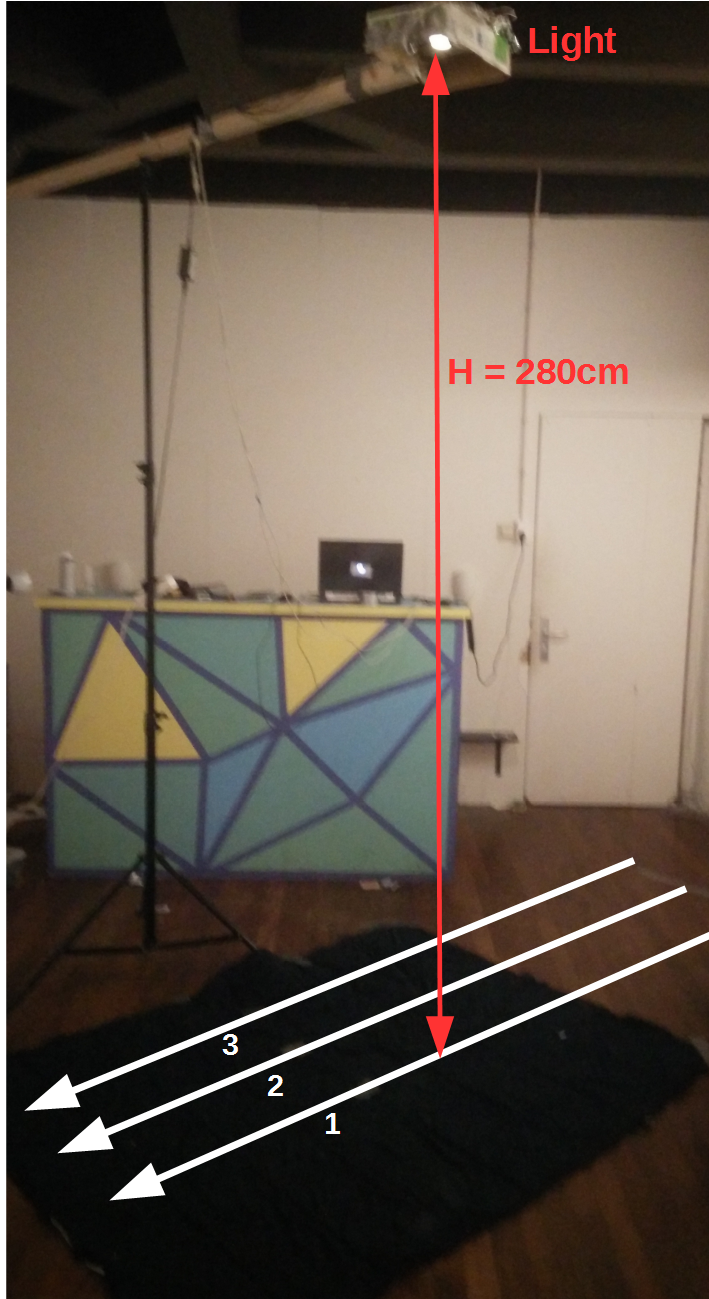
\includegraphics[width=50mm]{pics/Testsetup.png}}
	\subfigure[]{\label{fig:setup_b}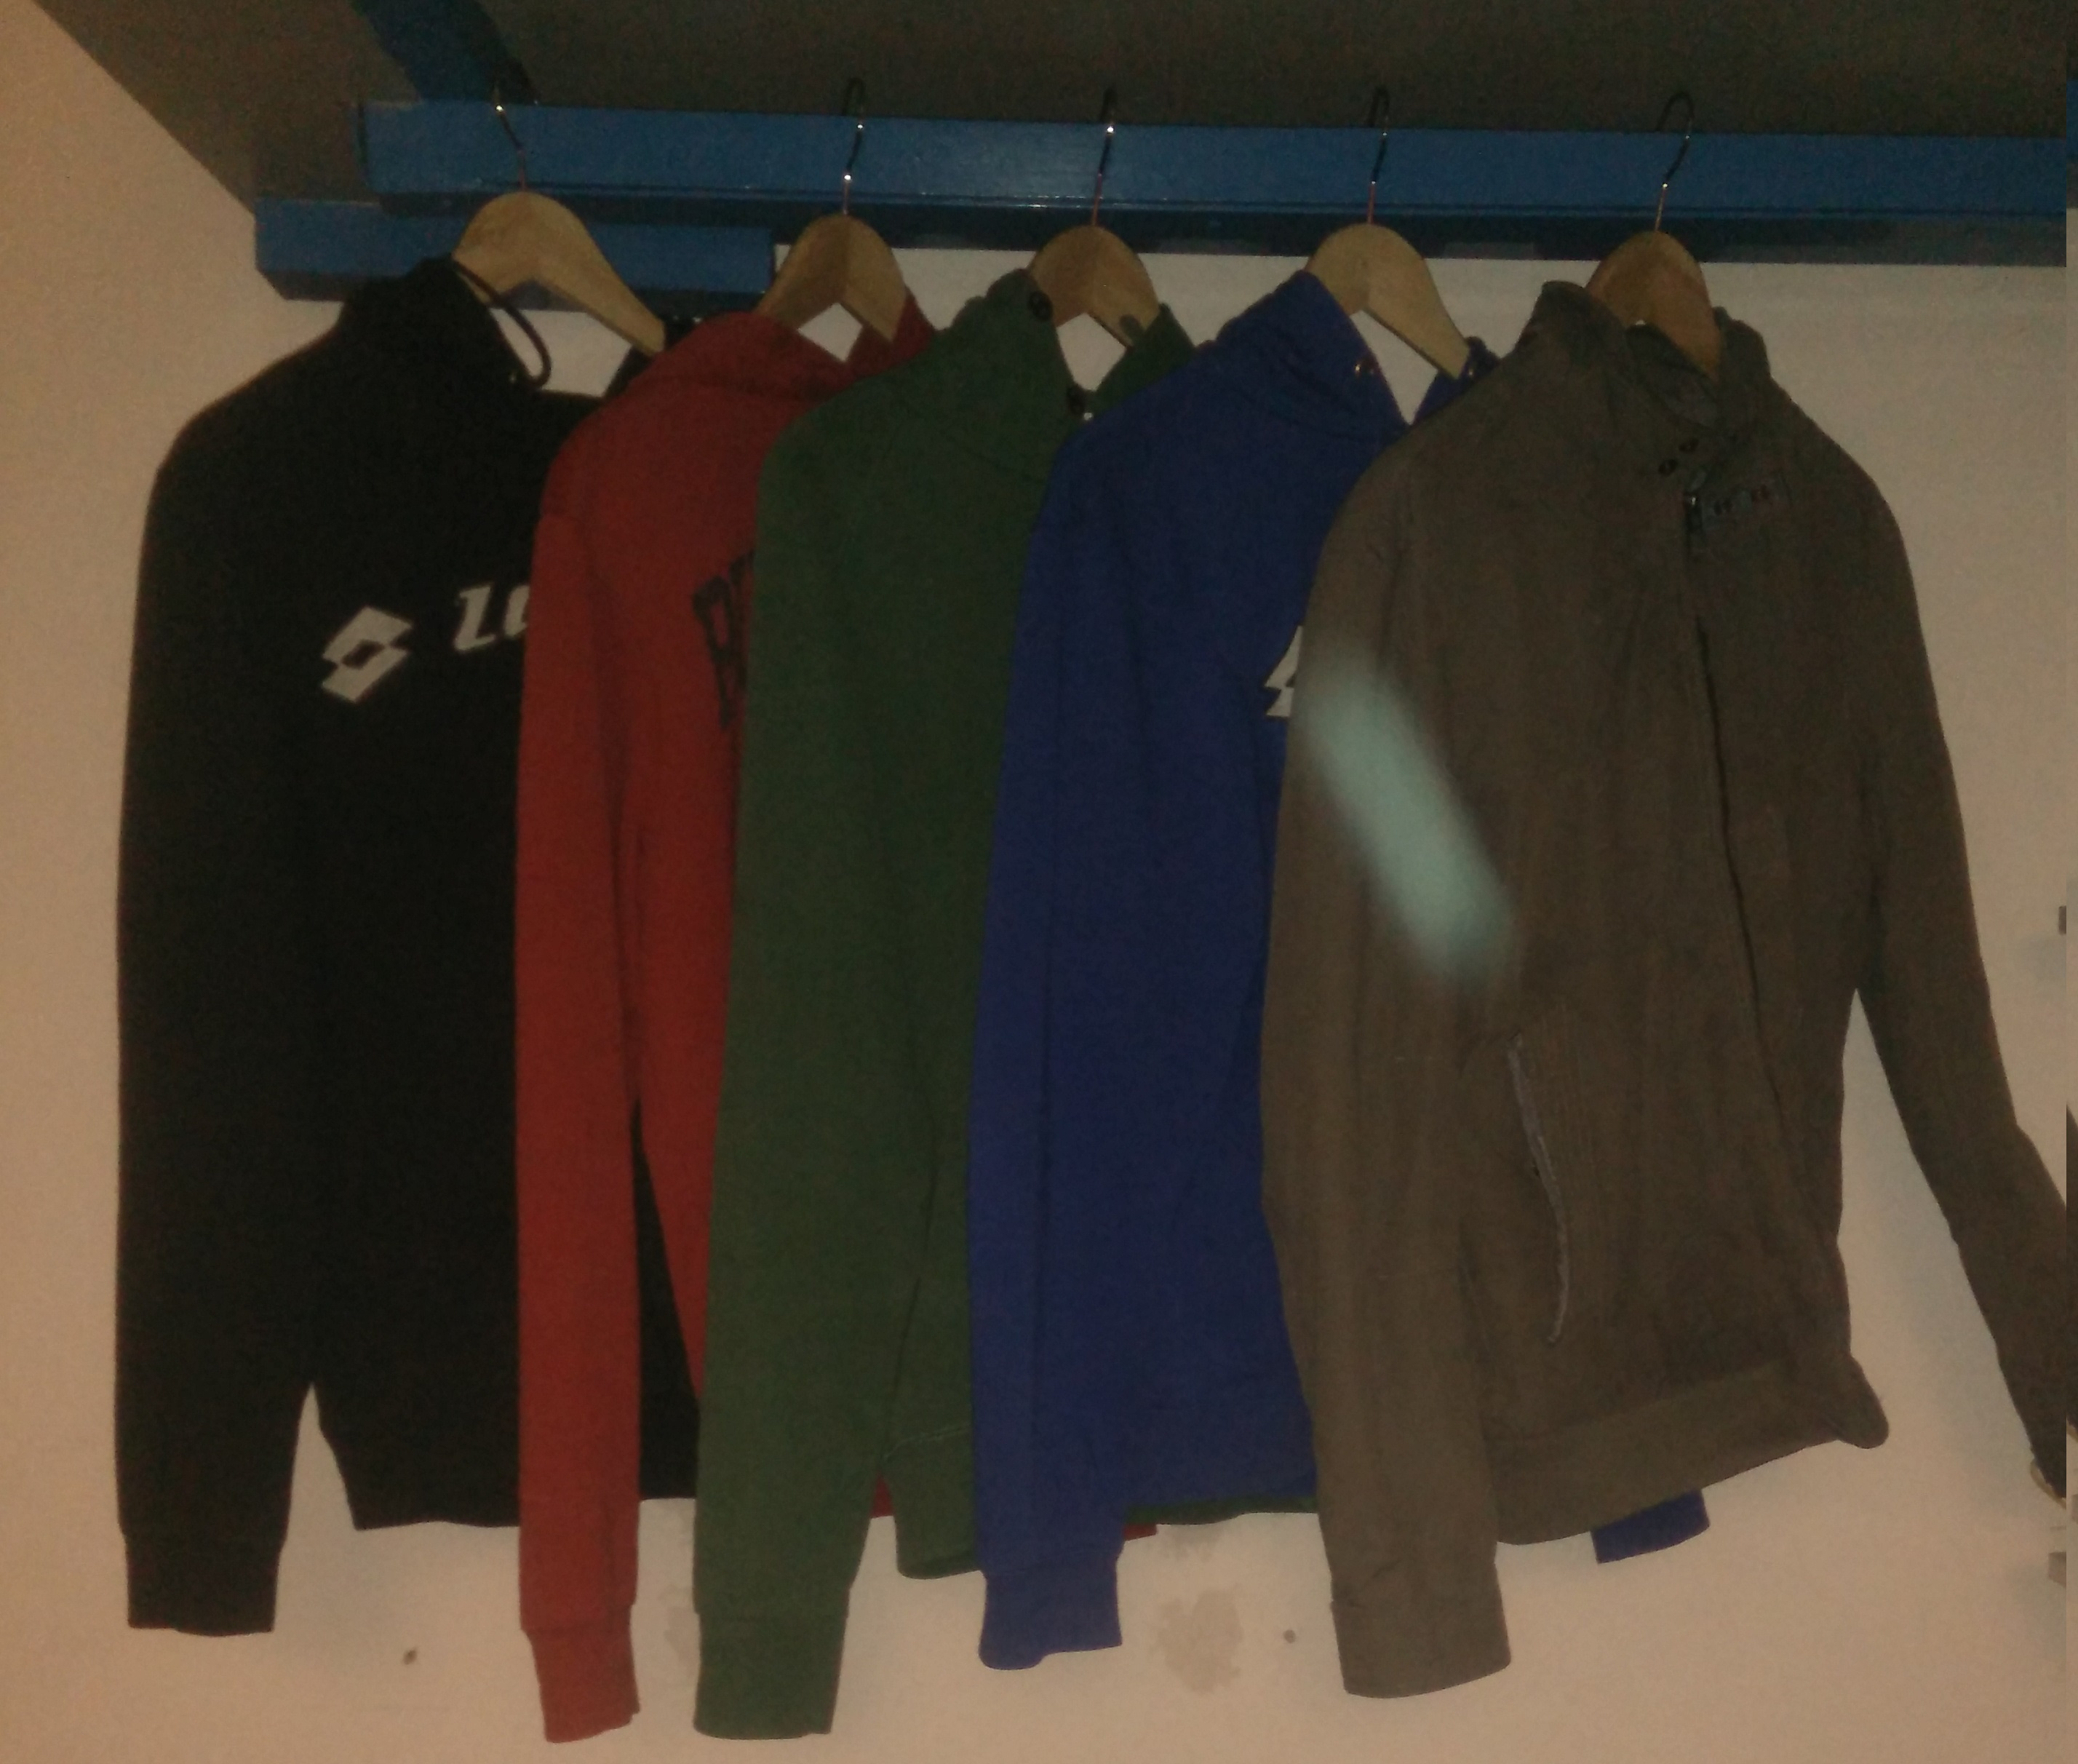
\includegraphics[width=70mm]{pics/Clothing.jpg}}
	\caption{(a) shows a picture of the test set-up with the blue carpet. The white arrows on the floor represent the three different paths the test subject walked over. The light is suspended at 2.8m. (b) shows the different clothing worn during the experiment (black, red, green, blue and grey).\label{fig:Testsetup}}
\end{figure}

\begin{figure}
	\centering     %%% not \center
	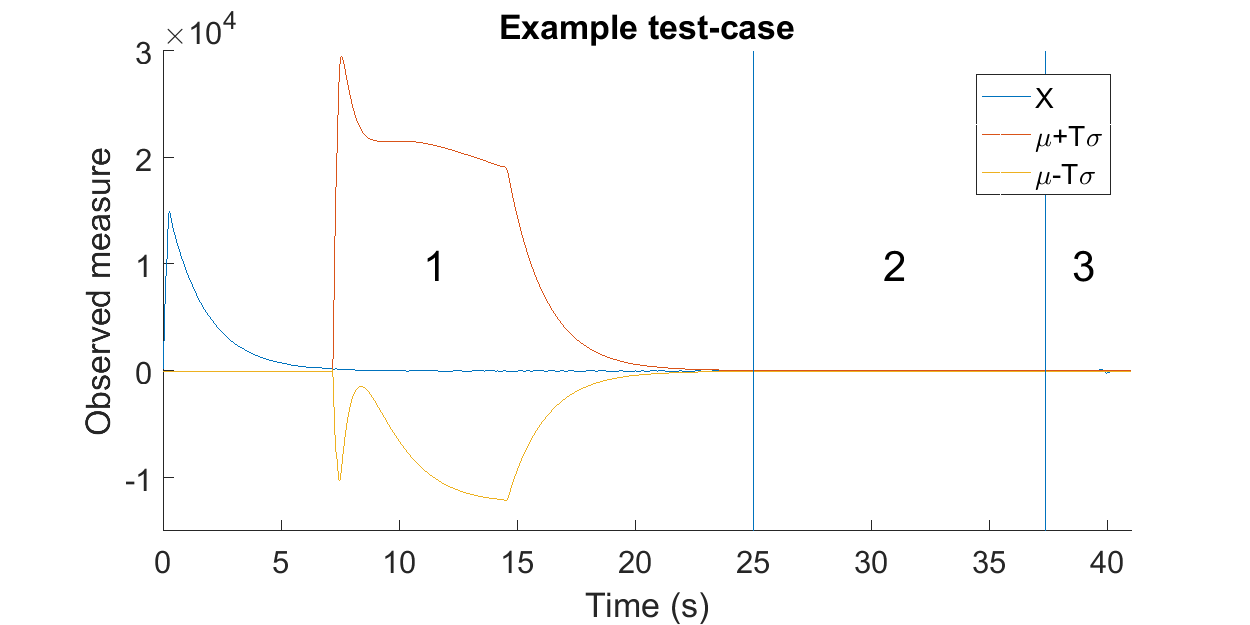
\includegraphics[width=\textwidth]{pics/Examplescenario.png}
	\caption{An example scenario with the tree sections marked.\label{TestScenario}}
\end{figure}
\section{Evolutionary algorithm}

\section{Results}

\section{Conclusion}
%Test setup
	% phisical setup
	% noise sources
	% 

%method of training: Evolution

%



%%%%%%%%%%%%%%%%%%%%%%%%%%%%%%%%%%%%%%%
In the previous chapter, two different algorithms where proposed, which could be capable of classifying a set of consecutive samples into two groups: Activity detected or no activity detected. The algorithms is however dependent on several values which have not been determined yet as they might, or might not be dependent on the operating environment. The goal of this chapter is to find a single set of settings for the algorithm which is capable to operate in several environments.

This chapter will start by finding several good settings for the algorithm with the help of an genetic algorithm. The best found algorithm will manually optimised for the application. The chapter will then finalise with evaluating the performance of the found settings.

\section{Algorithm settings}
Finding good settings for an algorithm can be a hard task, as depending on the algorithm, 5 or 6 values can be tweaked resulting in over $10^8$ different configurations. Testing all of the possibility is not feasible It was therefore chosen to us a evolutionary algorithm (EA) to find a reasonable setting for the created algorithms. An EA needs two things in order to work:
\begin{enumerate}[itemsep=-1ex,topsep=0pt]
	\item A fitness function, capable representing the performance of the algorithm in one value.
	\item A dataset, with labelled events which the fitness function can use to evaluate the performance of the algorithm.
\end{enumerate}
This section will first show how the labelled dataset was created and will then explain how this dataset was used to evaluate the fitness of an proposed algorithm. It finishes by presenting three algorithms obtained with the evolution process.

\subsection{The labelled dataset}
Two datasets where created to evaluate each potential algorithm. Both datasets where made with the system suspended 280cm above the ground and having a person walk underneath the light while sampling values. The only difference between the two data sets is the material of the ground the light is reflecting off of. The first set was created with a lacquered wooden floor while the other set was created with blue carpet. The difference between the two used surfaces lies in their reflection properties. The wooden floor has some specular component, where the carpet is almost fully diffuse. An overview of the setup can be seen in Figure \ref{fig:setup_a}.

Each datasets contains 15 different scenarios of how a person passes by the light. These scenarios are created by adjusting the colour of the clothing of the pedestrian and the path they take while walking past the light. The colour of the pedestrian was adjusted by making him wear different colour clothing (see Figure \ref{fig:setup_b}). Three different paths where marked on the ground which the test-subject had to walk over. The three paths where placed 30cm apart from each other with the first path placed directly under the light and the second and third paths lying 30 and 60cm from the center of the light. These paths are shown in Figure \ref{fig:setup_a}.

Each scenario was repeated 6 times, resulting in a dataset of 90 testable sequences. The dataset was labelled while capturing a scenario. The capture procedure of one scenario was done in the following manner:
\begin{enumerate}[itemsep=-1ex,topsep=0pt]
	\item Position the persons at the beginning of a path.
	\item Start the system, and make the person wait for $\pm35$ seconds.
	\item Tell the person to start walking, when the persons starts walking, label that sample as the start of an event.
	\item When the person stops walking (after he has passed the light), stop the sampling.
\end{enumerate}
This procedure created a consistent dataset for the EA to use. The first 25 seconds of a scenario are the time required for the algorithm to calibrate its filters and determine the moving mean and standard deviations. The next 10 seconds serve to detect if the system wrongly classifies silence as an event. The final 5 seconds of scenario is where the actual event happens.

\begin{figure}
	\centering     %%% not \center
	\label{fig:TestPicture}
	\subfigure[]{\label{fig:setup_a}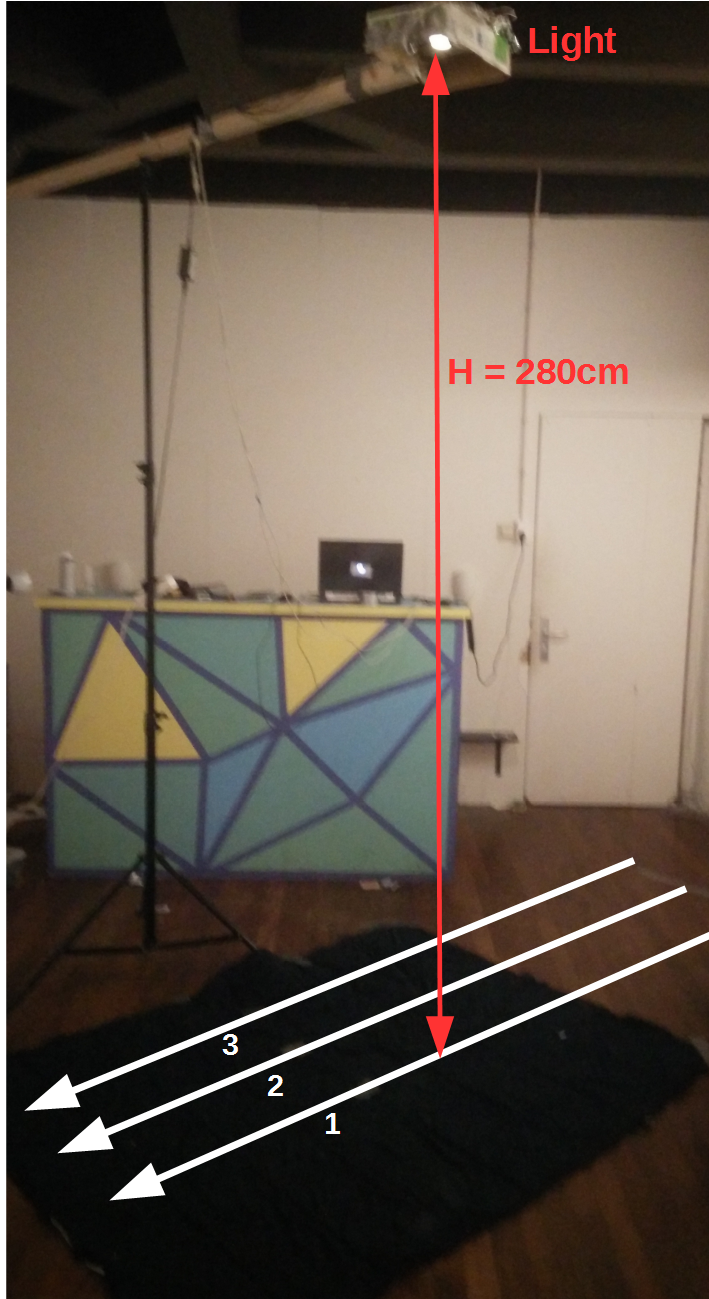
\includegraphics[width=50mm]{pics/Testsetup.png}}
	\subfigure[]{\label{fig:setup_b}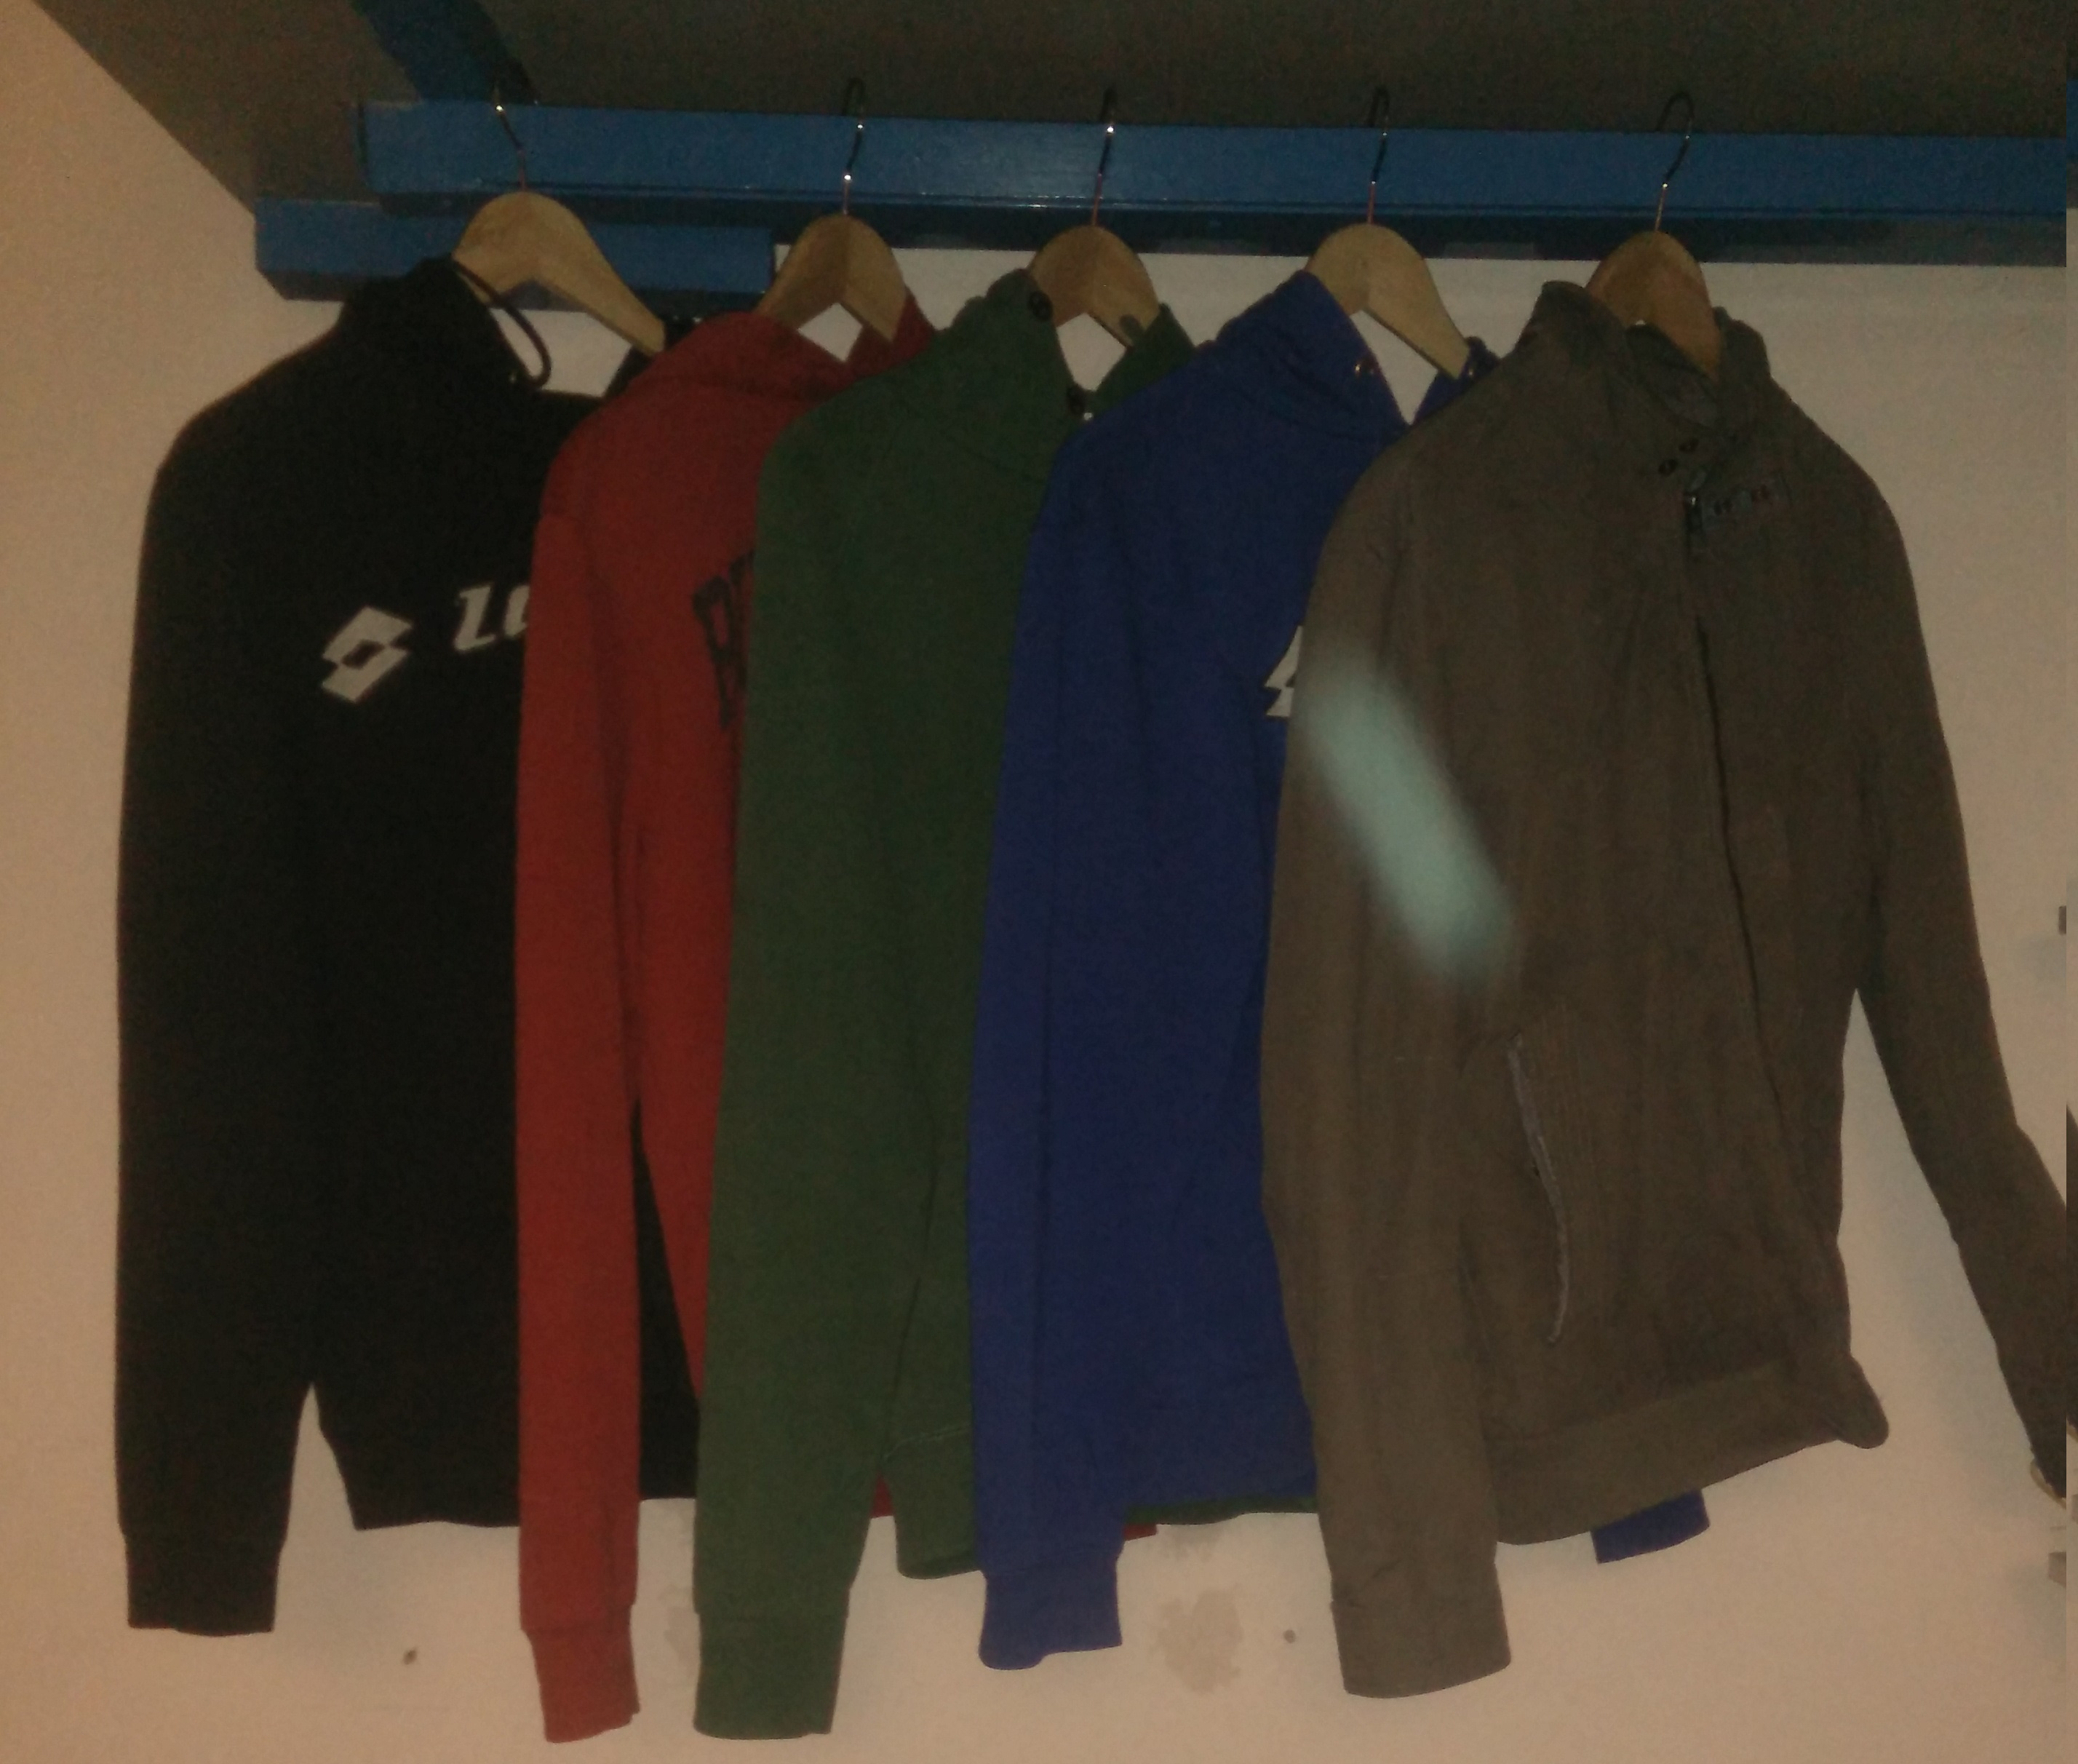
\includegraphics[width=70mm]{pics/Clothing.jpg}}
	\caption{(a) shows a picture of the test set-up with the blue carpet. The white arrows on the floor represent the three different paths the test subject walked over. The light is suspended at 2.8m. (b) shows the different clothing worn during the experiment (black, red, green, blue and grey).\label{fig:Testsetup}}
\end{figure}

\begin{figure}
	\centering     %%% not \center
	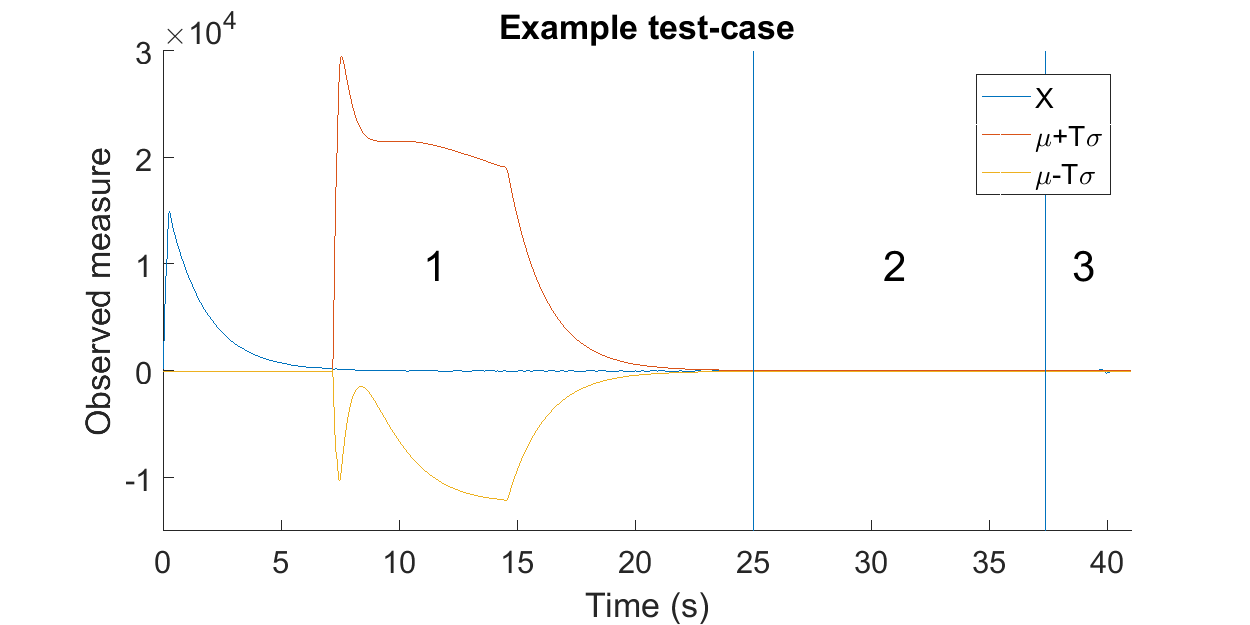
\includegraphics[width=\textwidth]{pics/Examplescenario.png}
	\caption{An example scenario with the tree sections marked.\label{TestScenario}}
\end{figure}

\subsection{The fitness function}
A fitness function was created to properly evaluate any proposed algorithm for a set of scenarios. The function evaluates an algorithm with the following rules for each scenario in the set:
\begin{itemize}[itemsep=-1ex,topsep=0pt]
	\item The algorithm \textbf{correctly} classifies an event as an event (True positive)$\rightarrow +1$
	\item The algorithm \textbf{incorrectly} classifies idle-time as an event (False positive)$\rightarrow -1$
	\item The algorithm does not detect an event $\rightarrow +0$
	\item The algorithm correctly classifies the event but also claims that the idle-time before anything happens is an event $\rightarrow +0$
\end{itemize}
Using this function, each proposed algorithm will get a penalty value from $-n$ to $n$, where $n$ is the number of scenarios which where evaluated by the function.

\subsection{Evolutionary results}
The evolutionary algorithm was used to find 3 algorithms with both methods. Two where trained trained with $S_1$, another two where trained with $S_2$ and the final two where trained with both sets. All found algorithms where then tested against the other data sets. Results of these tests can be seen in Table \ref{tbl:evo}.

\begin{table}[]
	\centering
\begin{tabular}{l|lll|lll|lll}
	& \multicolumn{3}{c|}{$S_1$} & \multicolumn{3}{c|}{$S_2$} & \multicolumn{3}{c|}{$S_{12}$} \\ \hline
	Algorithm    & TP    & FP    & Fitness    & TP    & FP    & Fitness    & TP      & FP     & Fitness    \\ \hline
	STD $S_1$    & 87    & 3     & 84         & 81    & 11    & 70         & 168     & 14     & 154        \\ \hline
	STD $S_2$    & 81    & 2     & 79         & 81    & 5     & 76         & 162     & 7      & 155        \\ \hline
	STD $S_{12}$ & 87    & 4     & 83         & 81    & 8     & 73         & 168     & 12     & 156        \\ \hline
	VAR $S_1$    & 79    & 1     & 78         & 80    & 15    & 65         & 159     & 16     & 143        \\ \hline
	VAR $S_2$    & 78    & 0     & 78         & 77    & 12    & 65         & 155     & 12     & 143        \\ \hline
	VAR $S_12$   & 78    & 2     & 76         & 80    & 11    & 69         & 158     & 13     & 145       
\end{tabular}
	\caption{Results of the evolutionary algorithm.\label{tbl:evo}}
\end{table}

It can be seen that the STD algorithm greatly outperforms the VAR algorithms. From the STD algorithms the one trained on both datasets (STD $S_{12}$) performs the best. For this reason, STD $S_{12}$ will be used for the main application.

\section{Algorithm evaluation}
This section focusses on optimising and evaluating the best found algorithm (STD $S_{12}$). The goal is to have 

This section will start with discussing the measures of evaluation. It will then optimise the algorithm, so it performs better in the application environment. Once optimised, the system will be evaluated with the newly found algorithm.

\subsection{Measures of evaluation}
The system will be evaluated on two criteria: Precision and recall. Precision is defined in equation \ref{eq:precsion/recall} and gives us insight in how many situations the light would turn on unnecessarily. A precision of 1 means that the system will never trigger a false detection. A Precision of 0 means that no matter what happens, the system will think that an event has happened.

Recall is defined in equation \ref{eq:precsion/recall} and gives us insight in how often the light fails to turns on when an object passes by. A precision of 1 means that all bypassing humans will be detected. A precision of 0 means that none of the bypassing humans is detected.
\begin{equation}
\label{eq:precsion/recall}
Precision = P = \frac{TP}{TP + FP}
\quad
Recall = R = \frac{TP}{TP + FN}
\end{equation}

The goal of our system is to save energy by not turning the light on. For this reason, the most important measure for evaluating the system is precision. If the precision of the system is 0.9, then the system has a 10\% chance of turning on if it's turned on for 10 seconds. This extrapolates to a 46\% chance on a false positive every minute ($(1-0.9^6)\cdot 100\%$). In contrast to precision, a low recall does not instantly ruin the system. Yes, it might not be ideal as several bypassing persons might not be detected, but the person can take a slight detour or wave their hands to turn on the lights.

\subsection{Algorithm tweaking}
Of all the algorithm settings, $T$ has to most direct influence on the precision and recall. A plot, showing the precision and recall as a function of $T$ can be seen in Figure \ref{fig:Precision_recall}. This Figure serves as a useful tool for finding the ideal trade-off between precision and recall. As can be seen, reaching the highest score for precision costs a lot recall. This is because several scenarios contain artefacts caused by the implementation of the analyser. One of such artefacts can be seen in figure \ref{fig:Failure} at 32 seconds. The mean of the signal suddenly rises, which will trigger a false detection if $T$ is lower than 12. 

At this point, a decision has to be made: How much of our detections are we willing to give up to prevent false positives from happening. In this case, the best way of preventing false positives is to create a new prototype, which does not produce artefacts as shown in figure \ref{fig:Failure}. This is however out of scope for this thesis. $T$ was therefore chosen to be 6, as this will still allow us to evaluate system at some fair level. A $T$ of 6 results in a precision of 0.95 and a recall of 0.88.

\begin{figure}
	\centering     %%% not \center
	\label{fig:Finetuning}
	\subfigure[]{\label{fig:Precision_recall}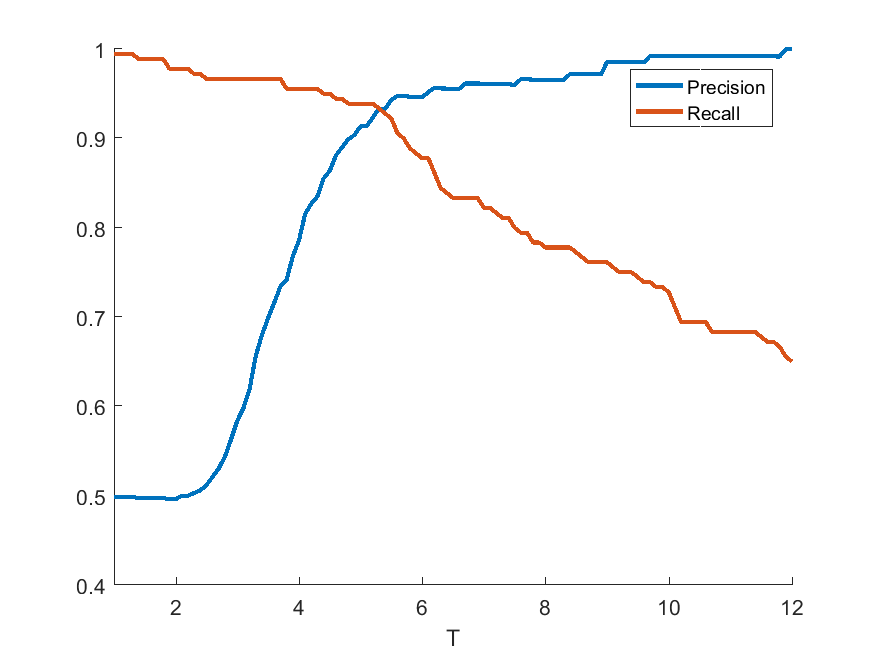
\includegraphics[width=60mm]{pics/Precision_Recall.png}}
	\subfigure[]{\label{fig:Failure}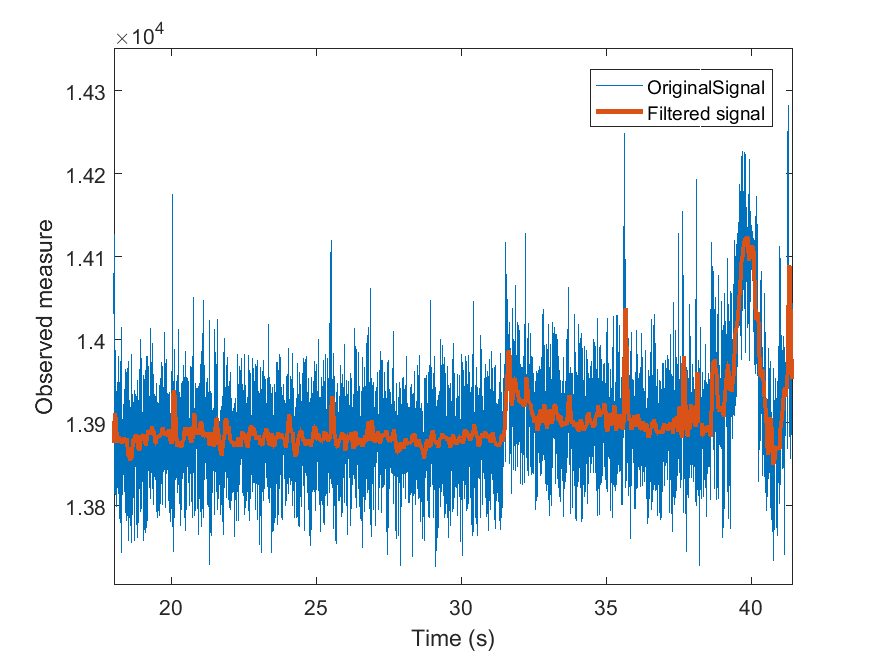
\includegraphics[width=60mm]{pics/ReasonForFailure.png}}
	\caption{(a) is a plot to see how the precision and recall change by increasing $T$. Precision won't reach 1 until $T = 12$. (b) shows an artefact causing a false positive.\label{fig:PnR}}
\end{figure}

\subsection{results}
The new algorithm was evaluated with the help of the created dataset. Table \ref{tbl:algresults} shows an overview of the results. It can be seen that all events taking place in lane one where detected. Lanes further away have a lower detection ratio. The system seems to have trouble detecting persons wearing black clothing once there person moves away from the centre of the light. This makes sense as black clothing typically absorbs more light than other colours.

The weak perception of the blue clothing can be explained by the LED used in the set-up. The actual colours emitted by the LED include fewer blue light than the light of other colours. Blue is however good visible when we walk upon the carpet. This is because the carpet has the same colour as the clothing. The carpet does not absorb most of the light reflected by the blue hoodie and is therefore very well visible by the system in the second dataset.

\begin{table}[]
	\centering
	\begin{tabular}{l|ccc|ccc}
		& \multicolumn{3}{c|}{Wooden floor}  & \multicolumn{3}{c|}{Carpet}        \\
		& Lane 1     & Lane 2    & Lane 3    & Lane 1     & Lane 2    & Lane 3    \\ \hline
		Red    & 6          & 6         & 6         & 6          & 3         & 5         \\
		Black  & 6          & 4         & 1         & 6          & 5         & 2         \\
		Green  & 6          & 6         & 6         & 6          & 5         & 6         \\
		Blue   & 6          & 6         & 3         & 6          & 5         & 5         \\
		Grey   & 6          & 6         & 6         & 6          & 6         & 6         \\ \hline
		Total: & 30 (100\%) & 28 (93\%) & 22 (73\%) & 30 (100\%) & 24 (80\%) & 24 (80\%)
	\end{tabular}
	\caption{Overview of the detection results with the found algorithm.\label{tbl:algresults}}
\end{table}
\emph{\color{red} Note for the proof reader: I wish I could add a section here which evaluates the system with the system without the training set. I however lack the time :(.} 
\\
\section{Conclusion}
This section has found a reasonable setting for the algorithm proposed in chapter \ref{chp:Analyser}. The settings where found by using an evolutionary algorithm over a realistic dataset. The found settings have been shown to be detect capable of detecting the pedestrian 88\% scenarios, no matter the colour, floor or path the person walked upon. The system however has a 26\% chance on a false positive every minute with the current settings.